\documentclass{article}
\usepackage{graphicx}
\usepackage{subcaption}
\begin{document}
	\section{Motivation}
	The programming language is python. The basic algorithm is the nearest centroid mean algorithm. The algorithm initially compute the mean for each class. The mean is a vector which is computed by averaging all features of training data. The algorithm compute the Euclidean distance between vector of mean trained by the classifier and vector of test data. 
	
	
	
	\section{Problem solution}
	\subsection{problem a}
	Two figures is generated by using \textit{PlotDecBoundaries()}. The CSV file 
	\begin{figure}[hbt!]
		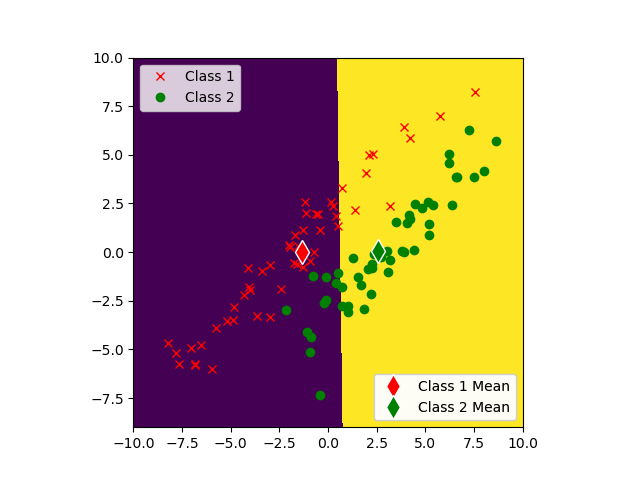
\includegraphics[width=\linewidth]{images/synthetic_trian1.png}	
		\caption{synthetic train1}
		\label{fig:synthetictrain1}
	\end{figure}
The Figure \ref{fig:synthetictrain1} shows the boundary is horizontal 
	\begin{figure}[hbt!]
		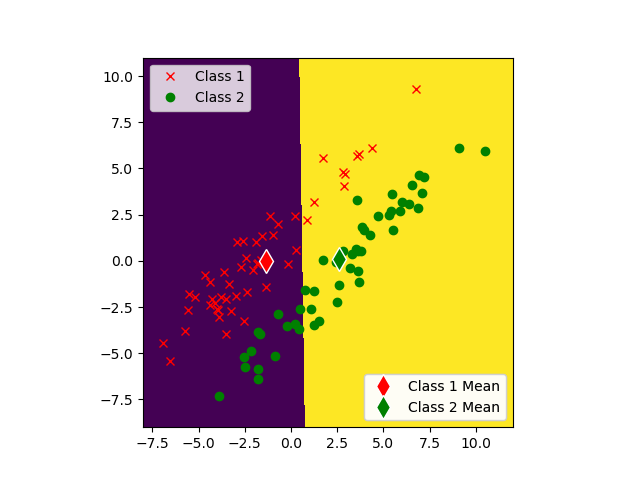
\includegraphics[width=\linewidth]{images/synthetic_test1.png}
		\caption{synthetic test1}
		\label{fig:synthetictest1}
	\end{figure}
	\begin{figure}[hbt!]
		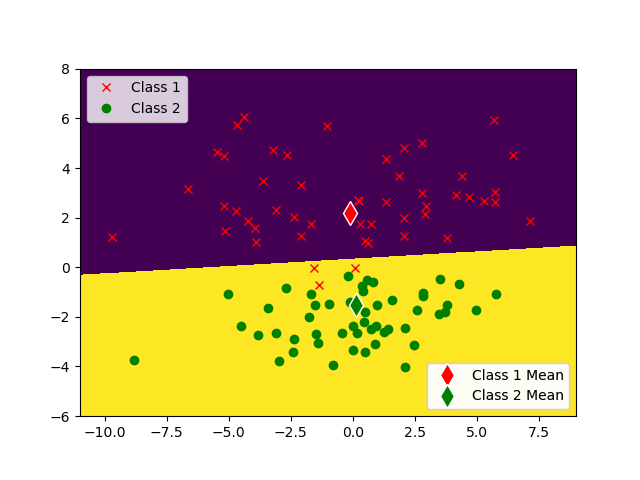
\includegraphics[width=\linewidth]{images/synthetic_train2.png}
		\caption{synthetic train2}
		\label{fig:synthetictrain2}
	\end{figure}
	\begin{figure}[hbt!]
		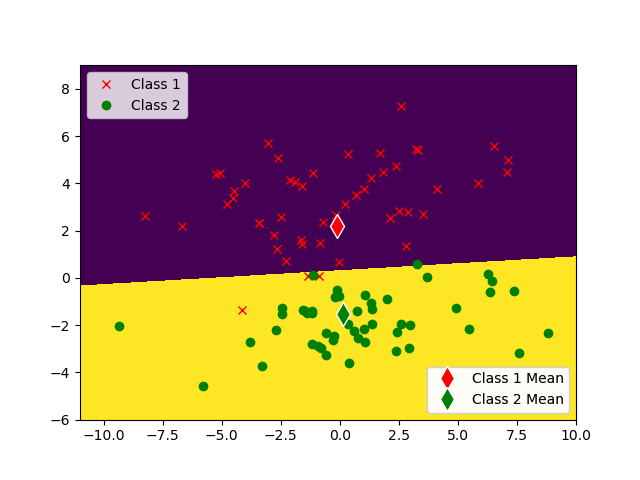
\includegraphics[width=\linewidth]{images/synthetic_test2.png}
		\caption{synthetic test2}
		\label{fig:synthetictest2}
	\end{figure}
		\begin{table}[hbt!]
		\begin{center}
		\begin{tabular}{| l | l | l | p{5cm} |}
		\hline
			Data      & Error rate & Test samples  \\ \hline
			synthetictrain1& 0.24        & 100    \\  \hline
			synthetictest1& 0.24		& 100    \\   \hline
			synthetictrain2& 0.04        & 100    \\  \hline
			synthetictest2& 0.04		& 100    \\   \hline
		\end{tabular}
		\end{center}
	\caption{Error rate}
	\label{table: errorrate}
	\end{table}
	 \\
	\subsection{problem b}
The error rate of both synthetic data set is the same. 
	\subsection{problem c}
		\begin{figure}[hbt!]
		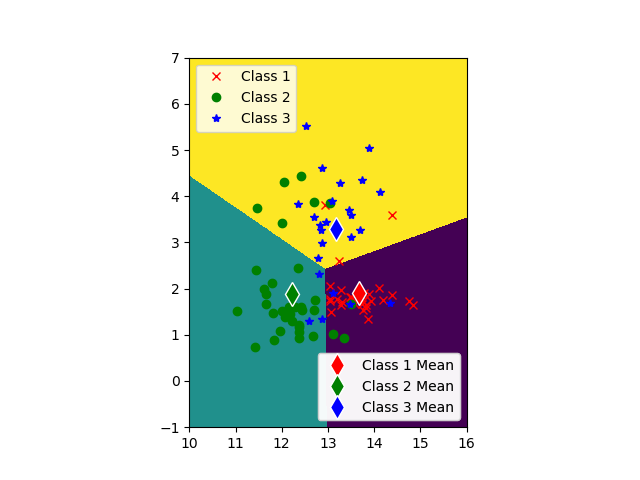
\includegraphics[width=\linewidth]{images/wine_feature01_train.png}	
		\caption{the data scatter plot of wine data set whose feature is 0 and 1}
		\label{fig:wine_feature01_train}
	\end{figure} 
	\subsection{problem d}
	\subsection{problem e}
	\section{Summary}
	
\end{document}